U komt in het werknemersscherm door in het hoofdmenu op de knop ``Werknemers''
te klikken.\\
\\
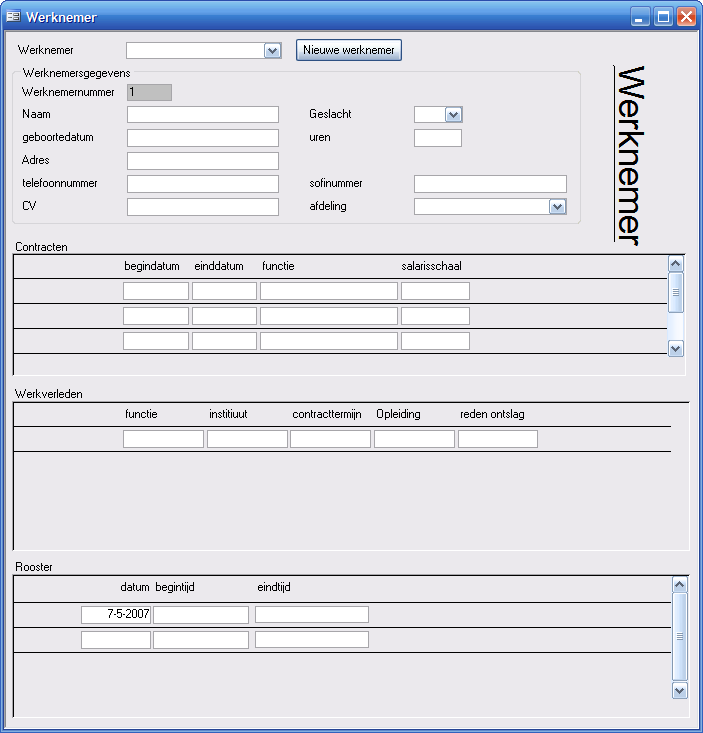
\includegraphics[scale=.5]{werknemer2} \\
\\
Selecteer bovenin het scherm een bestaande werknemer. U kunt ook een nieuwe werknemer aanmaken door op de ``Nieuwe
werknemer'' knop te klikken en vervolgens de juiste informatie in te voeren.

\section{Werknemersgegevens} \label{sec:werknemersgegevens}
    Onder het werknemersselectieveld staan de persoonsgegevens
    van de werknemer. Gebruik dit gebied om zaken als adresgegevens
    te wijzigen.

% subsection werknemersgegevens (end)

\section{Contracten} \label{sec:contracten}
    In het gebied ``contracten'' wordt op elke rij een contract
    van de werknemer bij het Zorgvliet Ziekenhuis weergegeven. Het
    huidige contract heeft geen einddatum. Om een contract toe te voegen, typt U de gegevens over dat
    contract in op de onderste regel. Er wordt dan automatisch een nieuwe lege regel aangemaakt.

% subsection contracten (end)

\section{Werkverleden} \label{sec:werkverleden}
    In het gebied ``werkverleden'' wordt op elke regel informatie over een
    opleiding of werkervaring van een werknemer buiten het Zorgvliet Ziekenhuis bijgehouden.
    Om een type werkervaring of opleiding toe te voegen, typt U de
    gegevens over die opleiding of werkervaring in op de onderste
    regel. Er wordt dan automatisch een nieuwe lege regel aangemaakt.

% subsection werkverleden (end)

\section{Rooster} \label{sec:rooster}
    In het gebied ``rooster'' wordt het rooster van een
    werknemer bijgehouden. Op elke regel staat een dienst van de
    werknemer. Om een dienst toe te voegen, typt U de gegevens in op een lege
    regel. Er wordt dan automatisch een nieuwe lege regel toegevoegd.

% subsection rooster (end)
